\documentclass[12pt,a4paper]{article}
\usepackage{listings}
\usepackage{hyperref}
\usepackage{graphicx}
\usepackage{float}
\usepackage{placeins}
\usepackage{subcaption}
\usepackage{amsmath}
\usepackage{cleveref}

\newcommand{\acomment}[1]{{\bf{\color{blue}{{[Aman: #1]}}}}}
\newcommand{\scomment}[1]{{\bf{\color{blue}{{[Suyash: #1]}}}}}

\hypersetup{
colorlinks=true,
allcolors=blue,
}

\usepackage{geometry}
\geometry{
a4paper,
left=20mm,
top=30mm,
}

\title{COL781: Computer Graphics\\Assignment 1}
\author{Suyash Agrawal (2015CS10262)\\Aman Agrawal (2015CS10210)}

\begin{document}
\maketitle
\section{Introduction}
    In this assignment we implement a ray-tracing module. We have implemented a recursive ray tracing algorithm principles as defined in the literature.
    
\section{Models}
    We have worked with the following models:
    \begin{enumerate}
        \item Sphere
        \item Quadric
        \item Plane
        \item Polygon
        \item Triangle
        \item Collection
        \item Box        
    \end{enumerate}

    All of these models, can be defined in their own local co-ordinate systems and need only the parameters required to define them completely.

\section{Lights}
    We have a functionality of specifying lights in the world co-ordinate system, and the color of the light emitted by them. Presently, all lights are point source.

\section{Camera}
    We presently have a support for specifying a single camera, and a transformation matrix, that specifies the lookat direction and position of the camera.

\section{Texture and Materials}
    We have a support of specifying texture for Sphere and Triangle. We find out the value of $u$ and $v$ for these models and map them to the texture image, to get the final color at the location in a texture map.\\\\
    \noindent We also, have a support of specifying a class of materials each with their own parameters, and each model object can be assigned a texture or a material.

\section{Ray Tracing}

    Finally, we perform a recursive ray tracing that renders the scene. Some of the samples of the rendered scenes are in \cref{fig:ray_tracing}
    

    \begin{figure*}
        \begin{subfigure}[ht]{0.475\textwidth}  
            \centering 
            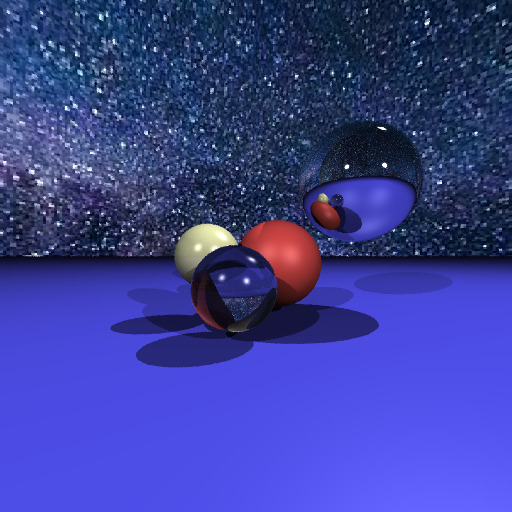
\includegraphics[width=\textwidth]{{imgs/spheres}.jpg}
            \caption{Spheres}    
        \end{subfigure}
        \hfill
        \begin{subfigure}[ht]{0.475\textwidth}   
            \centering 
            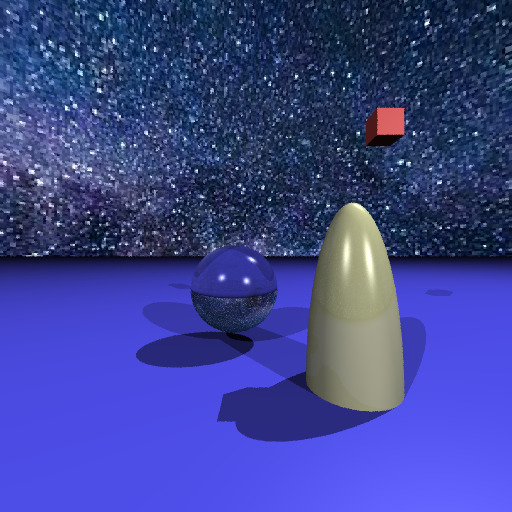
\includegraphics[width=\textwidth]{{imgs/box_quadric}.jpg}
            \caption{Box and Quadric}
        \end{subfigure}
        \vskip\baselineskip
        \begin{subfigure}[ht]{0.475\textwidth}  
            \centering 
            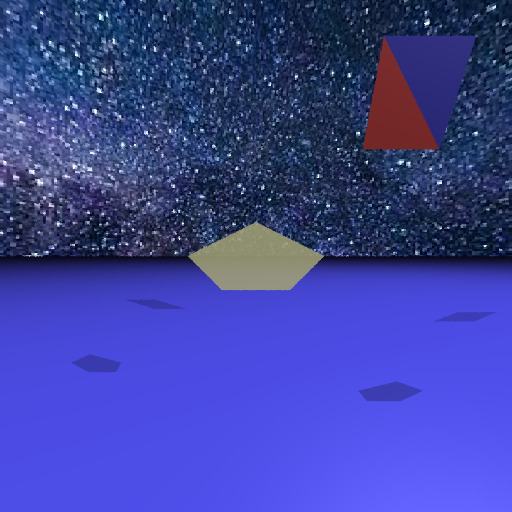
\includegraphics[width=\textwidth]{{imgs/polygon_collection}.jpg}
            \caption{Polygon and Collection}    
        \end{subfigure}
        \hfill
        \begin{subfigure}[ht]{0.475\textwidth}   
            \centering 
            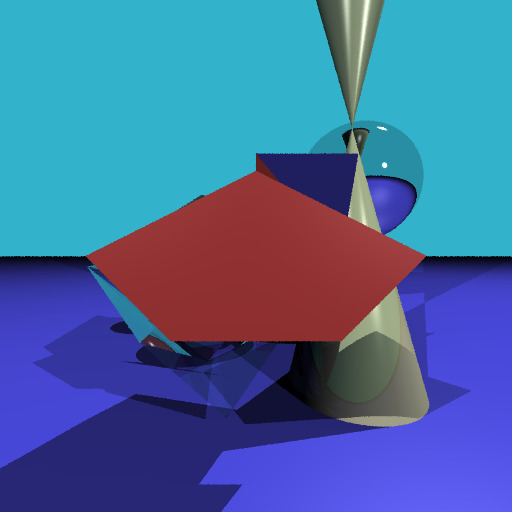
\includegraphics[width=\textwidth]{{imgs/all}.jpg}
            \caption{Complete Models}
        \end{subfigure}
        \caption{Results of Ray-Tracing with various models, and textures \label{fig:ray_tracing}}
    \end{figure*}

    \section{OpenGL Simulation}
    For OpenGL simulation we had to create new classes for our models. We created classes for Box, Sphere, Lights, Lines, Mesh and Camera.
    For the simulation we first re-drew our scene using the input json file and parsing them in our OpenGL model classes and then we calculated all the intersection lines using our ray traces code and drew these lines in OpenGL window. This gave us the required simulation of ray tracer for a given point in image.
    Some of the things like refraction and shadows were missing from our rendered scene since OpenGL uses rasterization instead of ray tracing and it is really tough to give shadows and refraction in rasterization.  
    We also made the camera system movable, thus giving us freedom to roam around the scene and explore the whole environment.
    See \cref{fig:opengl} for an example.
    \begin{figure*}
        \begin{subfigure}[ht]{0.99\textwidth}  
            \centering 
            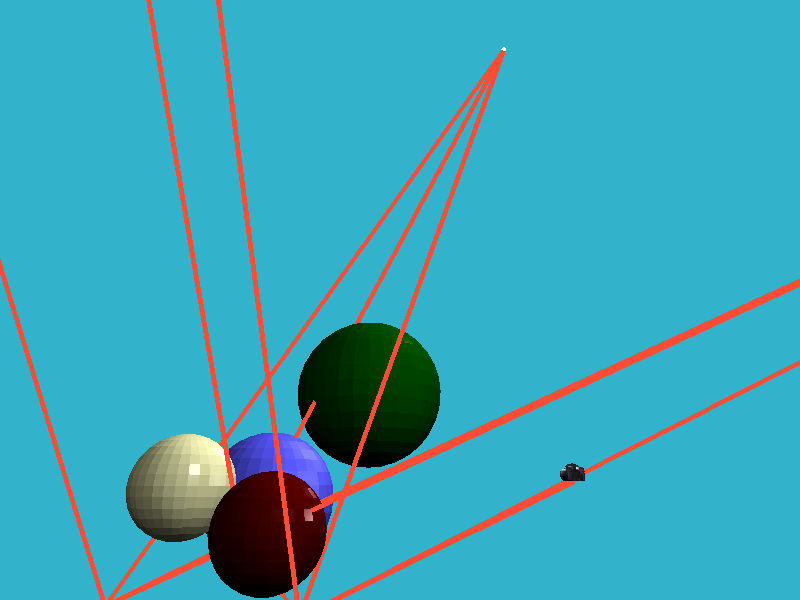
\includegraphics[width=\textwidth]{{imgs/opengl}.png}
        \end{subfigure}
        \hfill
        \caption{Results of OpenGL simulation \label{fig:opengl}}
    \end{figure*}

\end{document}
